\documentclass[12pt,letterpaper]{article}
\usepackage[utf8]{inputenc}
\usepackage[spanish]{babel}
\usepackage{amsmath}
\usepackage{amsfonts}
\usepackage{amssymb}
\usepackage{graphicx}
\graphicspath{{img/}}
\usepackage[left=2cm,right=2cm,top=2cm,bottom=2cm]{geometry}
\usepackage{apacite}
\usepackage{listings}
\author{Bryan Brenes}
\title{Proyecto final}

\renewcommand{\baselinestretch}{1.5}

\begin{document}
%Portada de documento
\begin{titlepage}
	\begin{center}
		{\large \textbf{Instituto Tecnológico de Costa Rica}} \\
		Escuela de ingeniería en computación \\
		Desarrollo de aplicaciones para dispositivos móviles\\
		IC-8066\\
		\vfill
		Proyecto 1: \\ Restaurantes\\
		\vfill
		Bryan Brenes Rojas - 201173608 \\
		Jean Pierre Monterrey Arguedas - 2016246285 \\
		Prof.: Andrei Fuentes Leiva\\
		\vfill
		Semestre I \\
		\today
	\end{center}
\end{titlepage}

\tableofcontents
\thispagestyle{empty}
\pagebreak

\section{Introducción}
Se desarrolla una aplicación en android para familiarizarse con el desarrollo en esta plataforma. A grandes rasgos, la aplicación debe permitir al usuario ingresar nuevos restaurantes donde se especifique información relevante entre esta la dirección que deberá ser mostrada en un mapa utilizando el API de Google para dicho fin. Además se debe poder listar y mostrar detalles de los restaurantes, así como poder realizar y visualizar comentarios del restaurante.

Se implementa además un backoffice para el manejo de las funciones de los administradores, así como un API para manejar el backend de la aplicación, lo que incluye el maneja de una base de datos en MongoDB y el manejo de consultas mediante el uso de json tanto para la solicitud como para el respuesta.


\section{Wireframes}
Con el objetivo de realizar la interfaz gráfica de la aplicación de una manera más precisa y eficiente se desarrollaron \textit{wireframes} donde se especifica la distribución de los elementos gráficos así como una idea de las proporciones que estos tendrán en cada una una de las pantallas de la aplicación.

\subsection{Pantalla inicial}
Esta es la primer pantalla que ve el usuario. Se muestran dos opciones posibles: registrarse o ingresar a la aplicación. Además se incluye una imagen que va a contener el logo principal de la aplicación. Cada una de las opciones tiene un botón asociado del cual registrarse se considera como el botón principal, dejando ingresar como botón secundario. En la fig.~\ref{img:pantalla_inicial} se muestra el \textit{wireframe} para esta pantalla.

\begin{figure}[h!]
	\begin{center}
		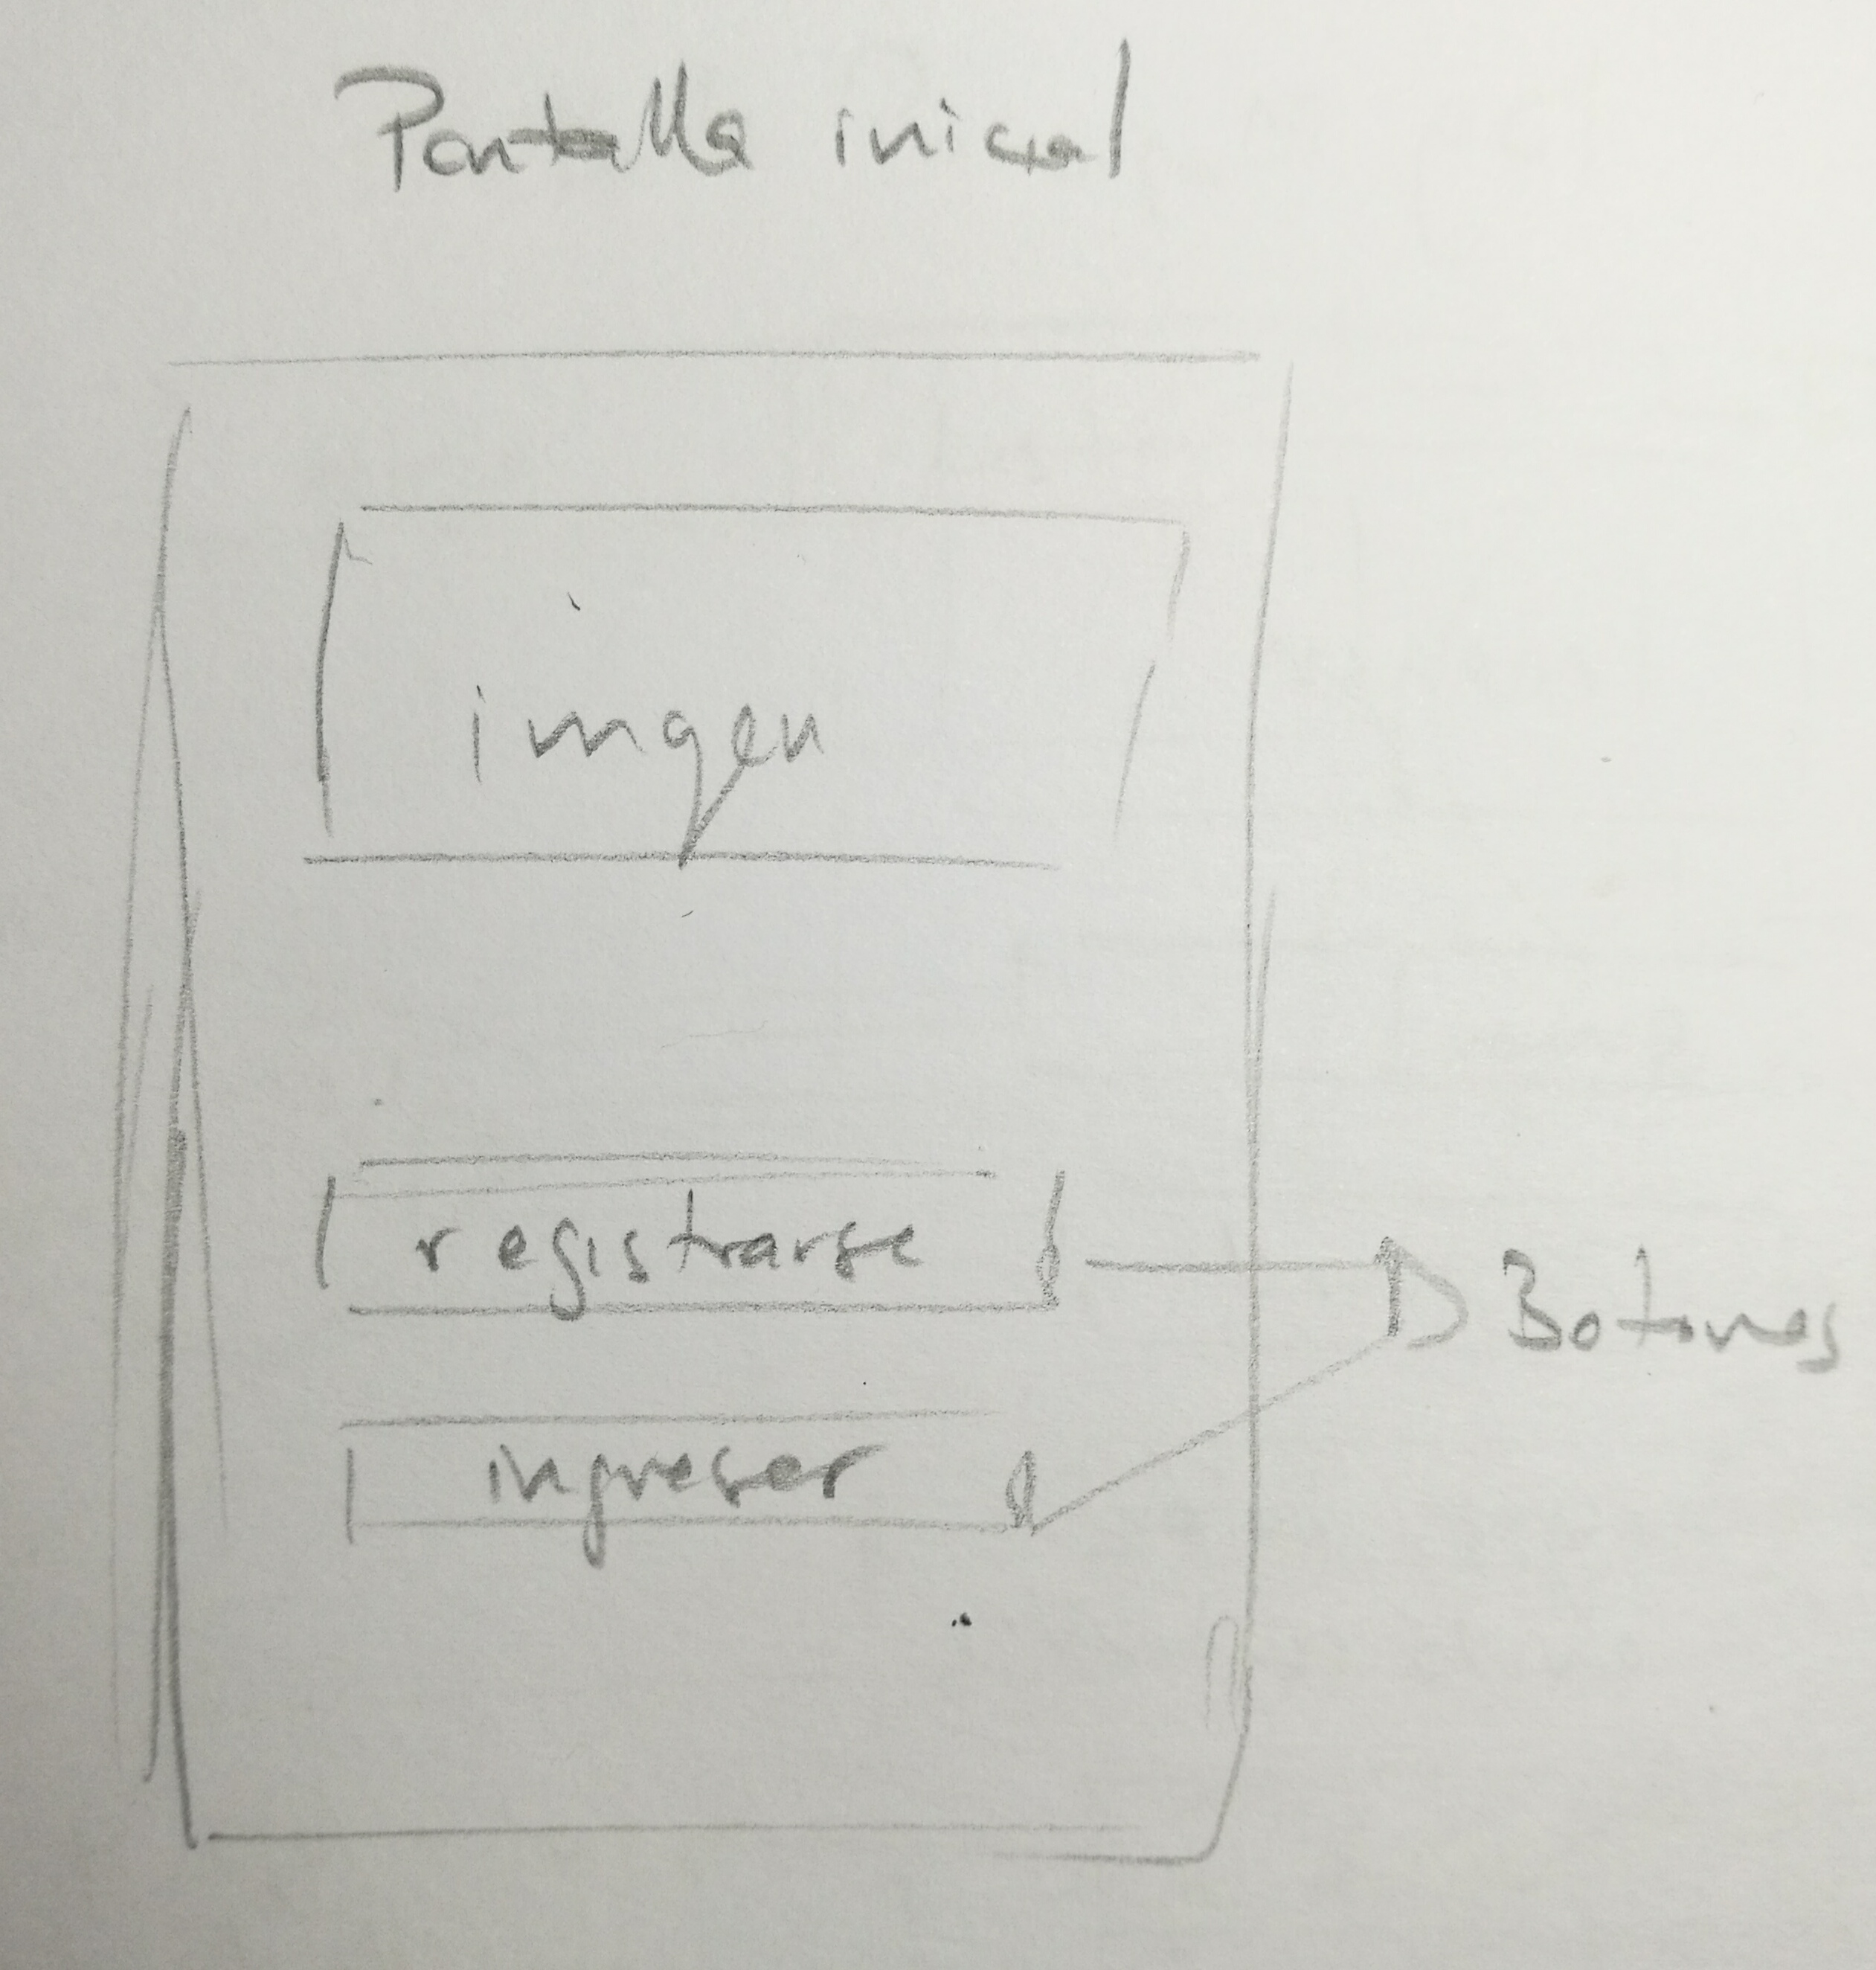
\includegraphics[scale=0.07]{pantalla_inicial.jpg}
		\caption{Pantalla inicial. Fuente: propia}
		\label{img:pantalla_inicial}
	\end{center}
\end{figure}

\subsection{Pantalla de registro}
Esta pantalla (fig.~\ref{img:pantalla_registro}) mantiene la misma imagen que la pantalla inicial de manera que dé uniformidad a la aplicación. La pantalla contiene la información necesaria para que el usuario pueda ser registrado en el sistema, esta información incluye el nombre de usuario, el correo electrónico, la contraseña y la confirmación de la contraseña. Por último se tiene el botón de registro.

\begin{figure}[h!]
	\begin{center}
		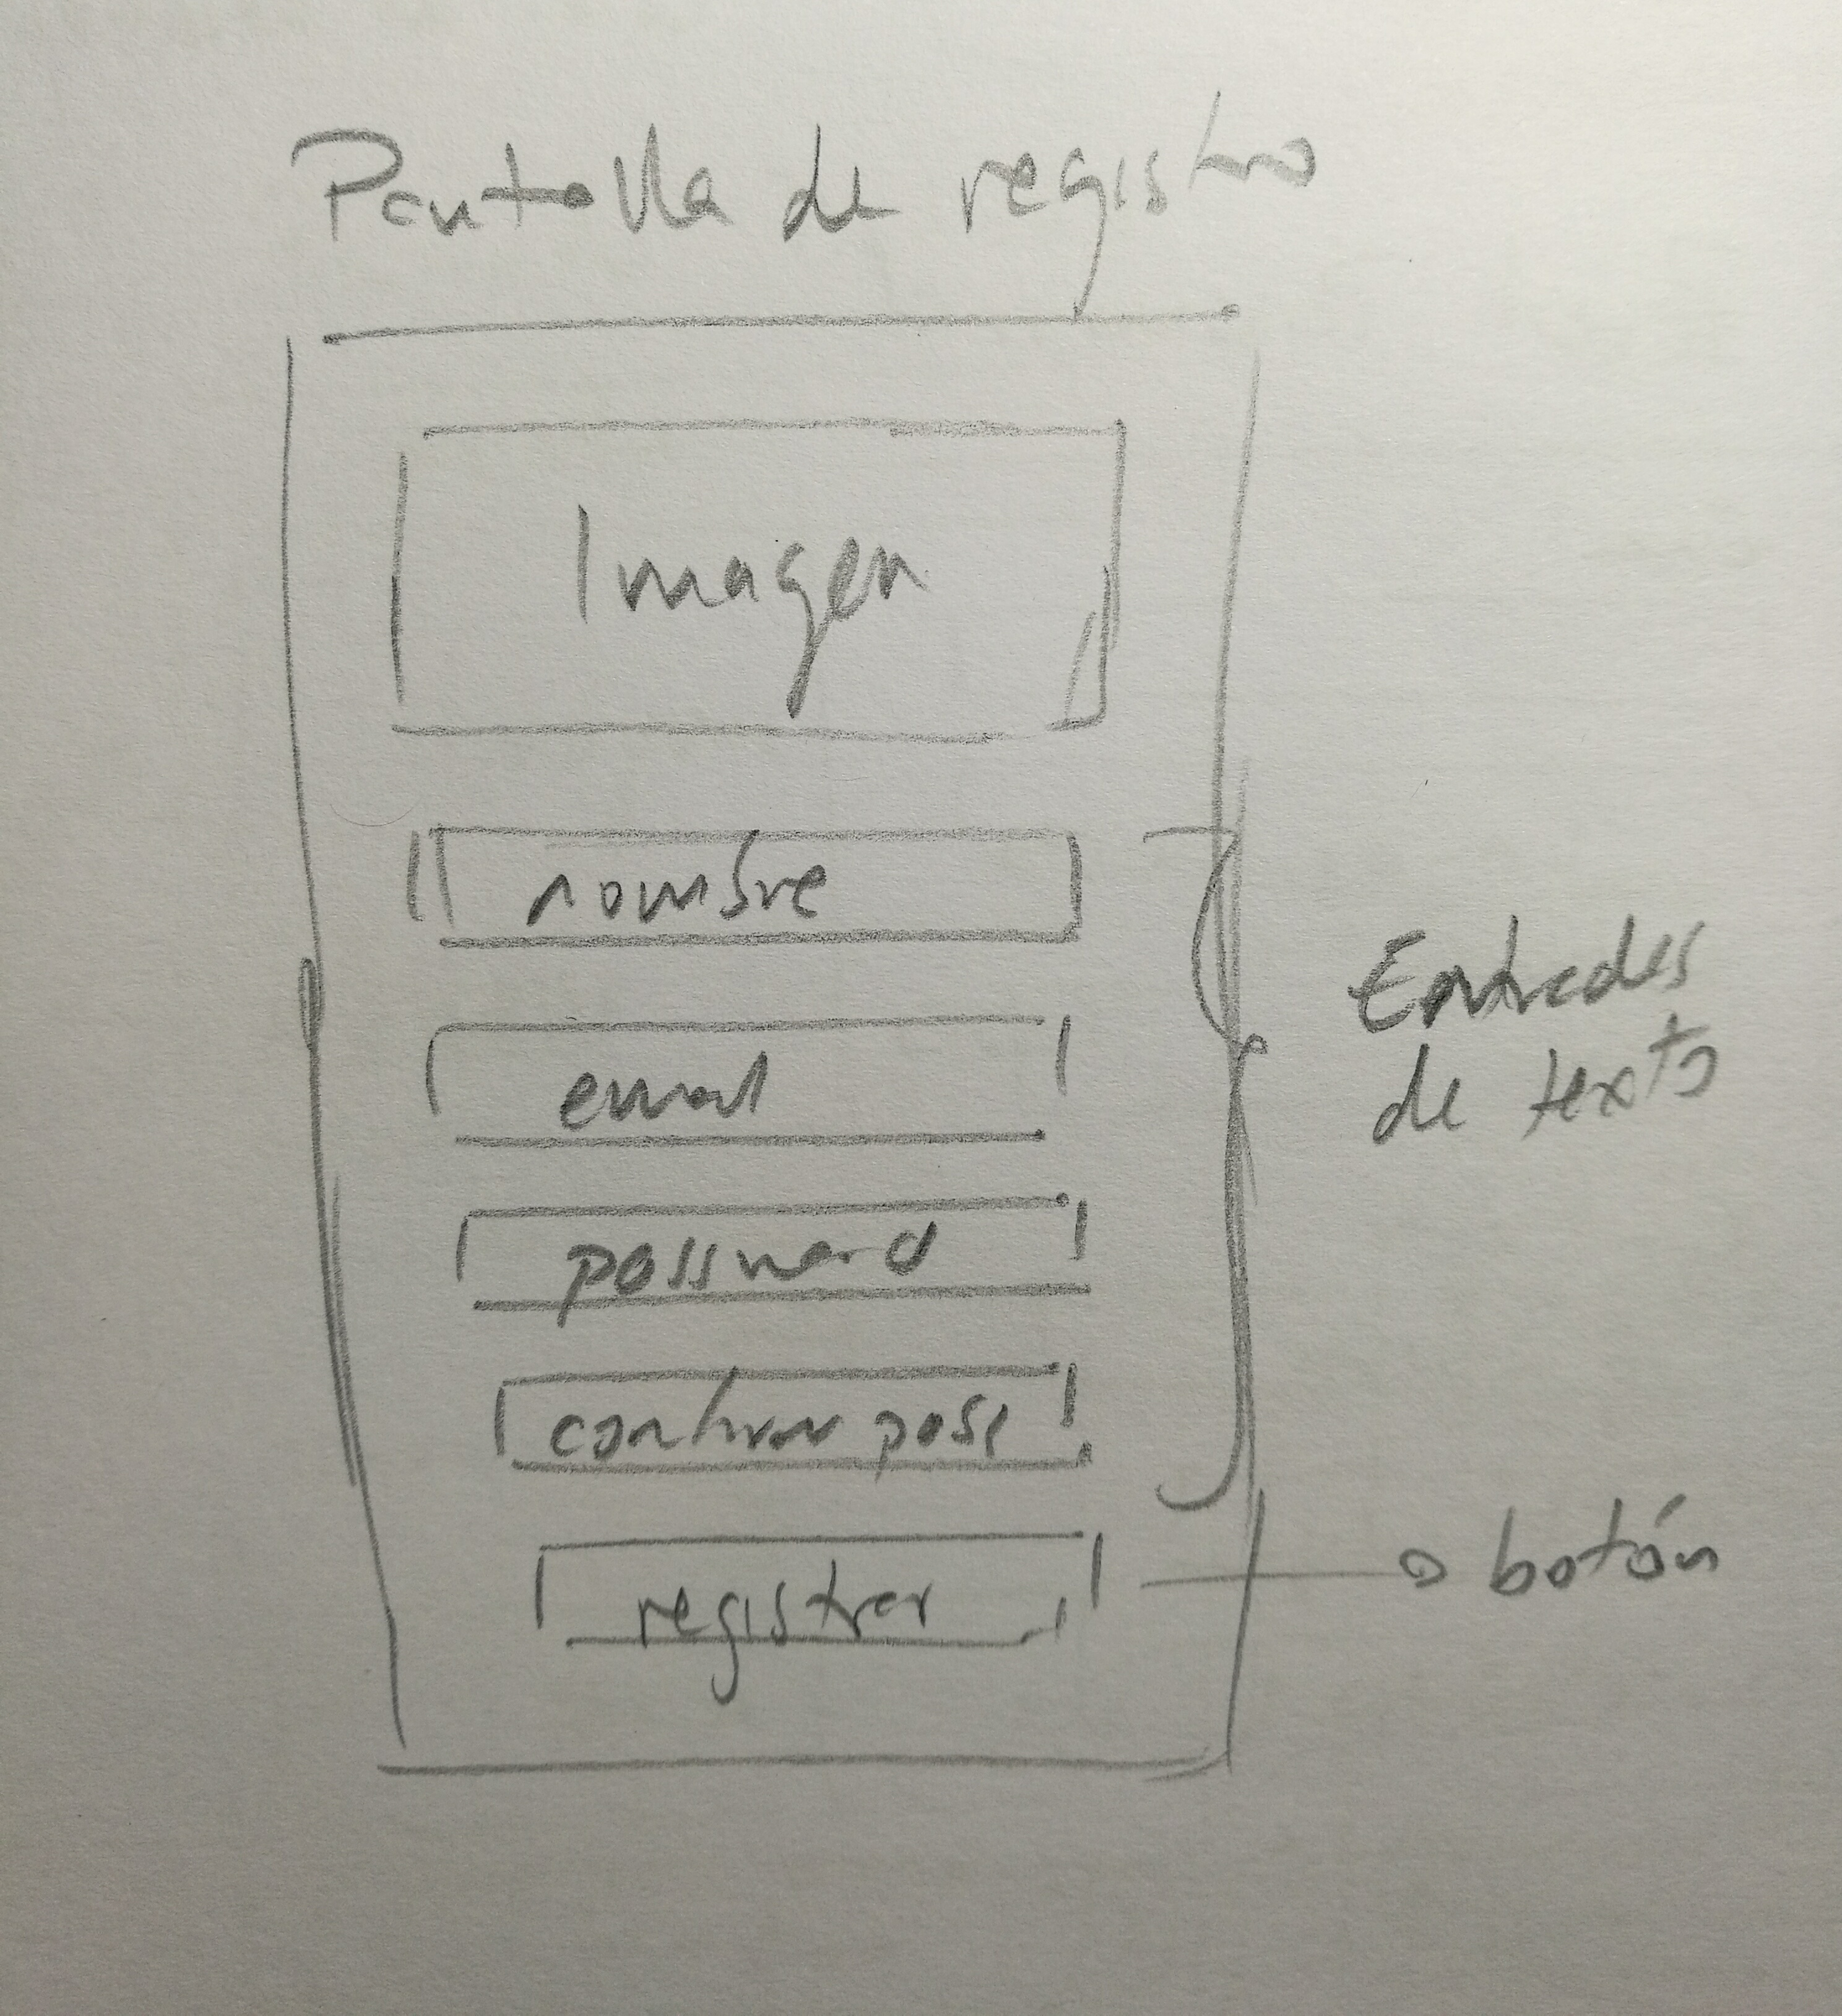
\includegraphics[scale=0.07]{pantalla_registro.jpg}
		\caption{Pantalla de registro de usuario. Fuente: propia}
		\label{img:pantalla_registro}
	\end{center}
\end{figure}

\subsection{Pantalla de login}
Para realizar el login se requiere del correo electrónico del usuario así como su contraseña, por esto en el \textit{wireframe} de esta pantalla que se encuentra en la fig.~\ref{img:pantalla_login} se muestran los campos para ingresar el correo y la contraseña. Además se incluyen la opción para realizar el log in y para restablecer la contraseña en caso de olvido.

\begin{figure}[h!]
	\begin{center}
		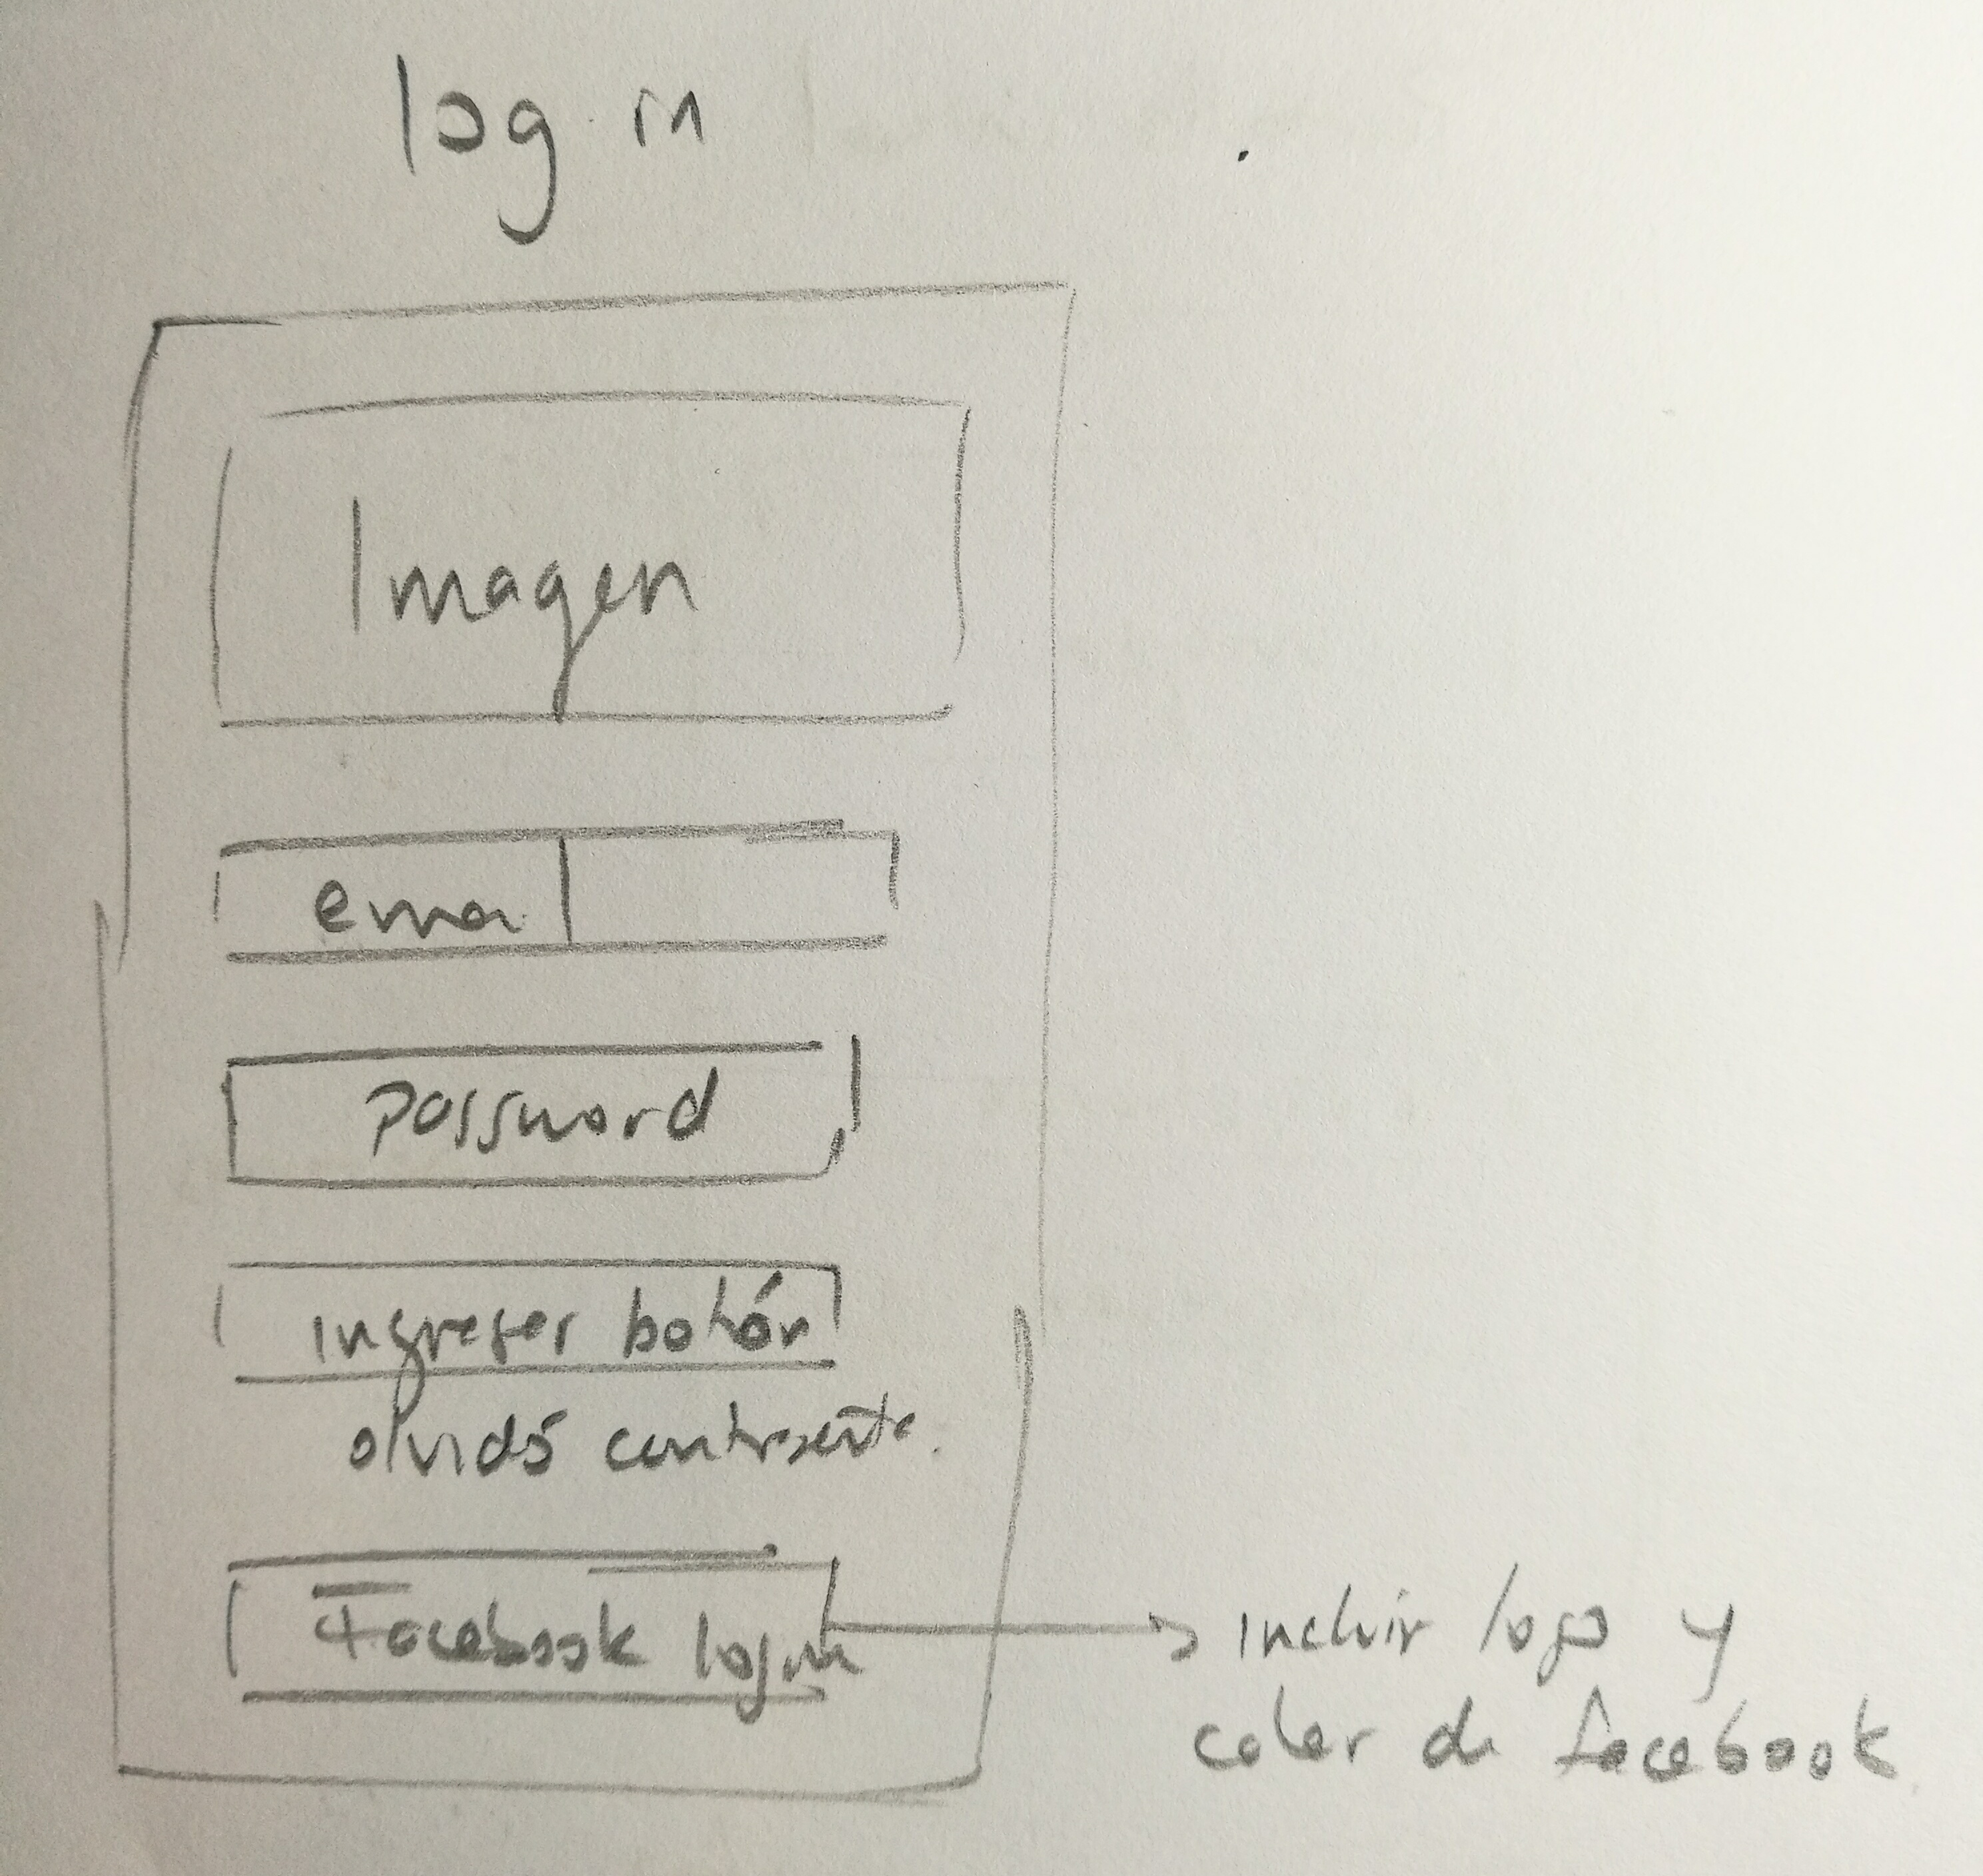
\includegraphics[scale=0.07]{pantalla_login.jpg}
		\caption{Pantalla de login de usuario. Fuente: propia}
		\label{img:pantalla_login}
	\end{center}
\end{figure}

\subsection{Pantalla de restablecimiento de contraseña}
En la fig.~\ref{img:pantalla_reset} se muestran los elemento gráficos requeridos para realizar este proceso. Se coloca un campo de texto para que el usuario ingrese el correo electrónico al cual se le va a enviar el correo así como un botón para realzar el envío. Se dispone además de campos para la nueva contraseña así como para la confirmación de esta. Por último se tiene campo para ingresar el código que es enviado por el correo.

\begin{figure}[h!]
	\begin{center}
		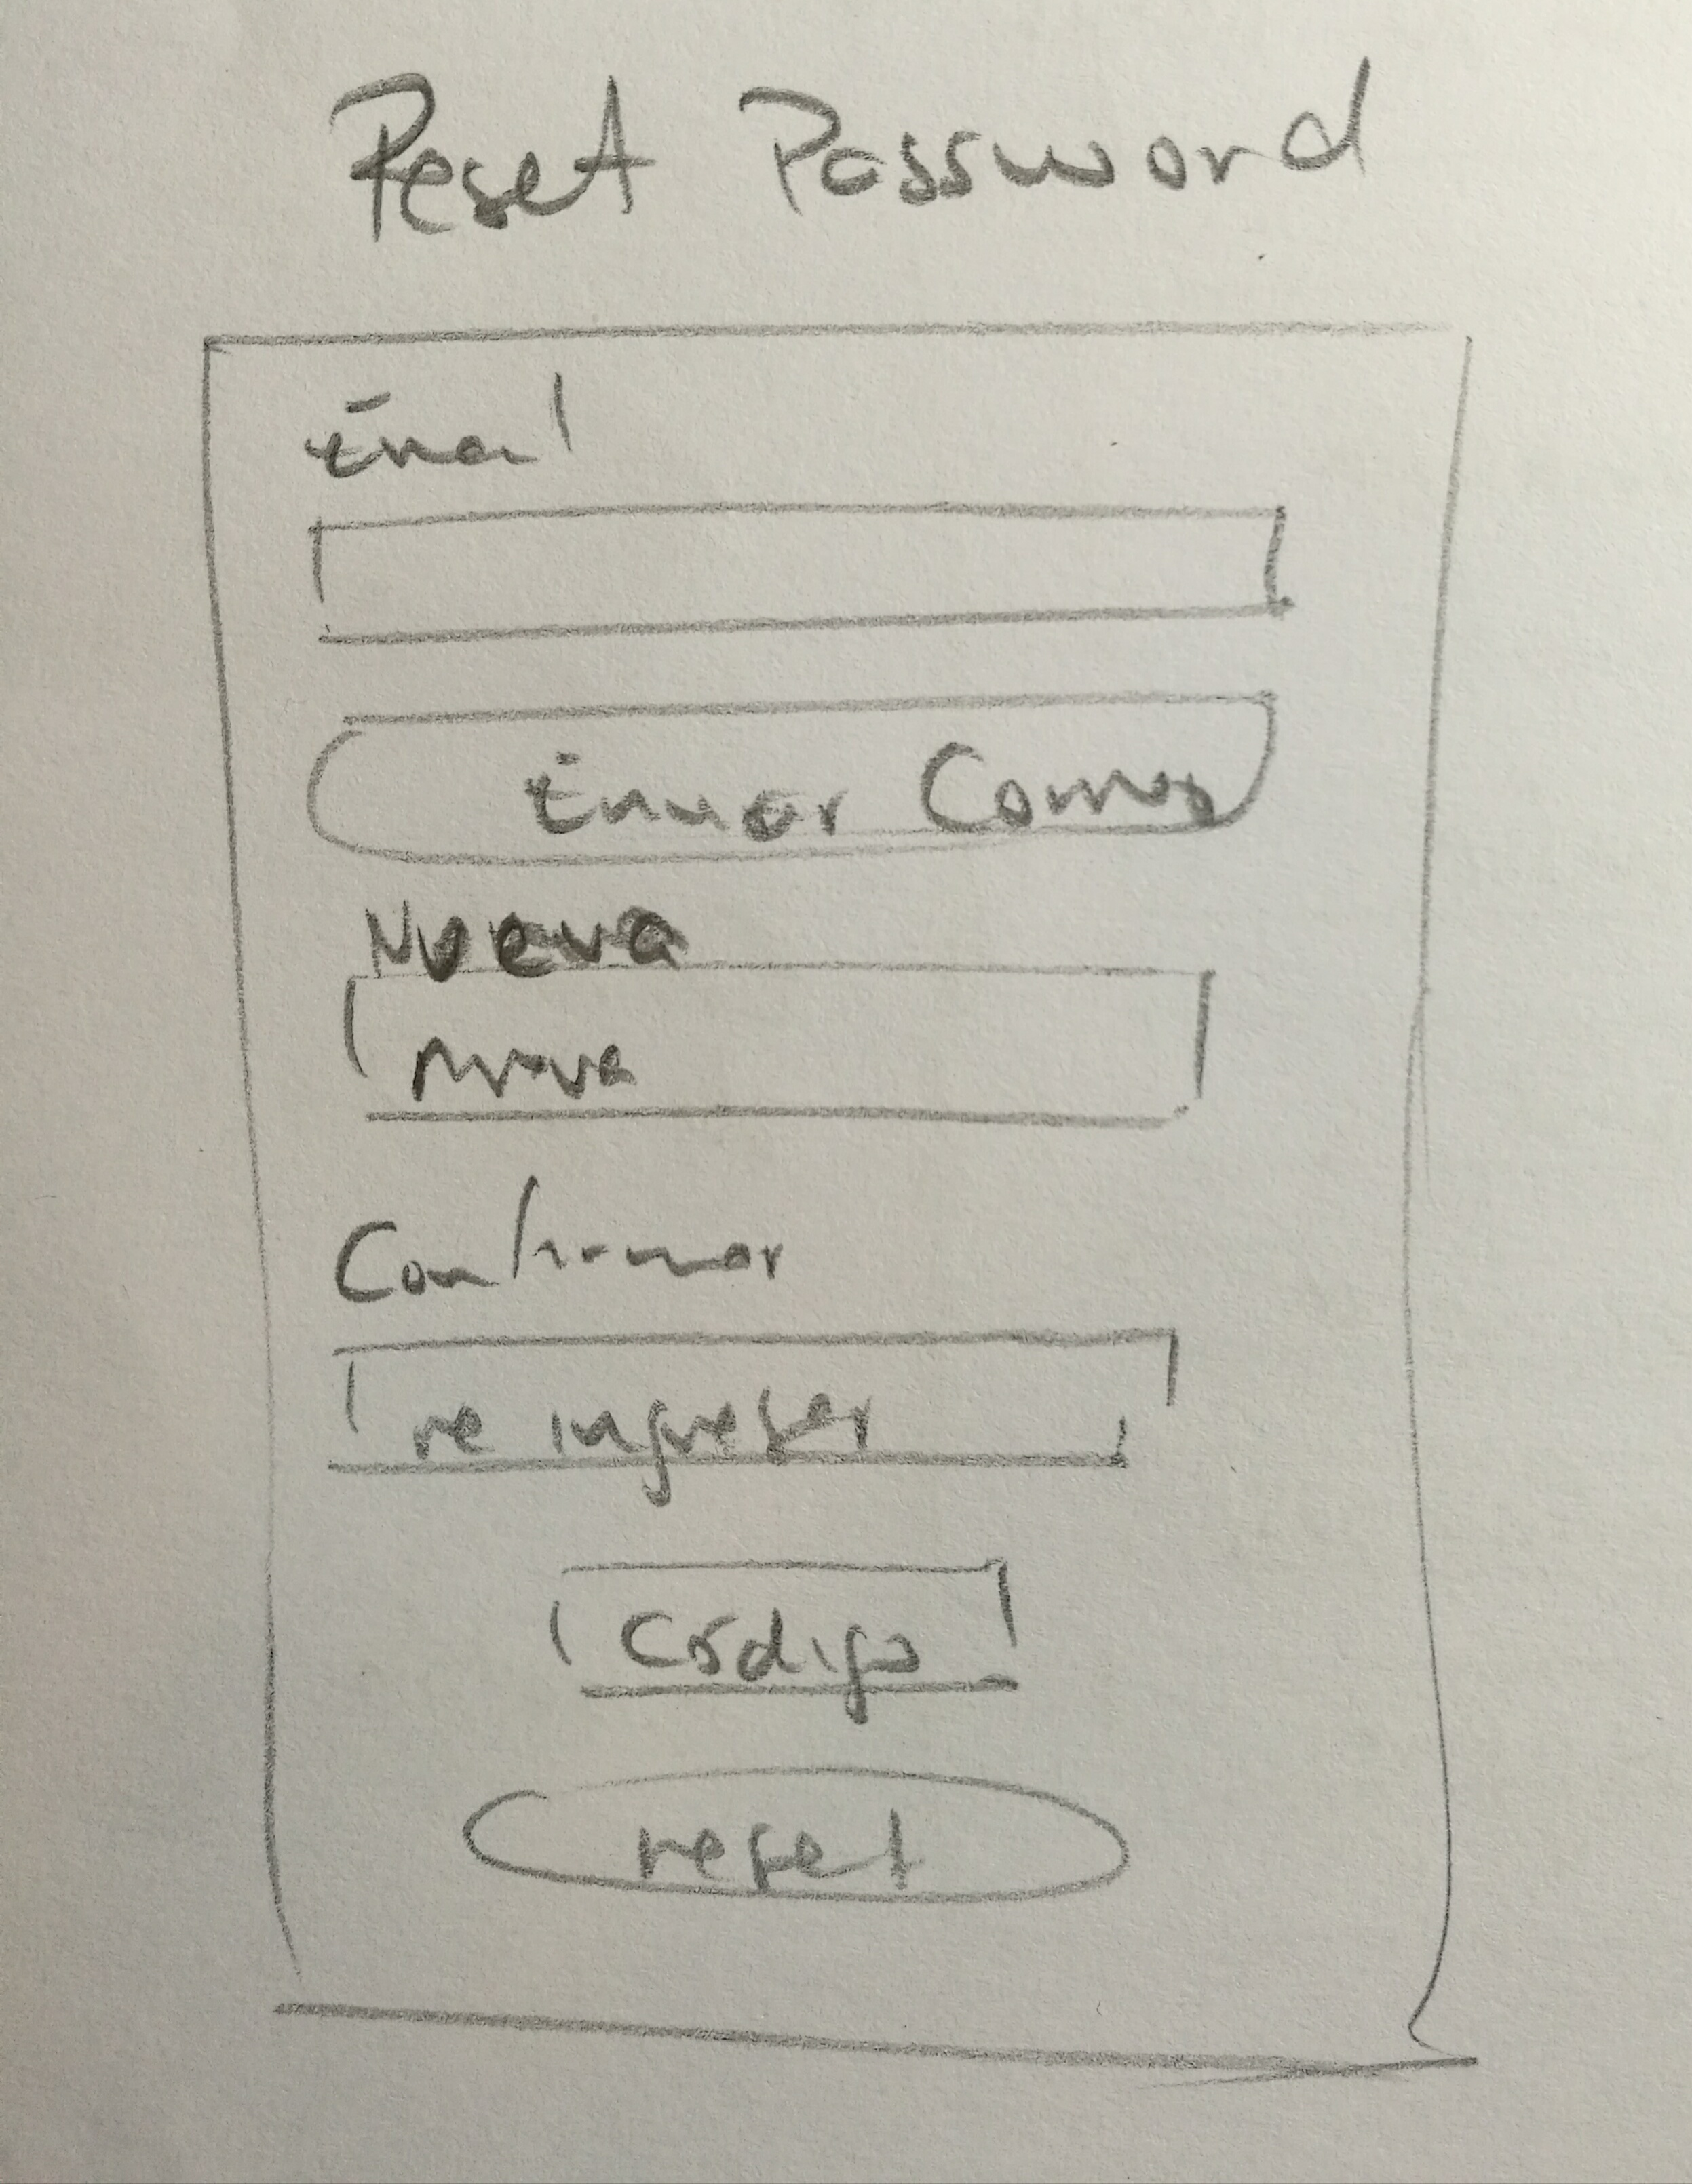
\includegraphics[scale=0.07]{pantalla_reset.jpg}
		\caption{Pantalla de restablecimiento de contraseña. Fuente: propia}
		\label{img:pantalla_reset}
	\end{center}
\end{figure}

\subsection{Pantalla principal}
La pantalla principal de la aplicación esta diseñada utilizando pestañas de manera que se tiene dos vista como se muestra en la fig.~\ref{img:pantalla_principal}. Una de las pestañas tiene la vista del mapa con las ubicaciones de los restaurantes, mientras que la otra pestaña tiene un lista de todos los restaurantes, en esta lista se maneja un formato para cada uno de sus ítemes, como se muestra en el \textit{wireframe} se tiene una imagen del restaurante, nombre y ubicación, así como una imagen para mostrar la calificación del restaurante.

\begin{figure}[h!]
	\begin{center}
		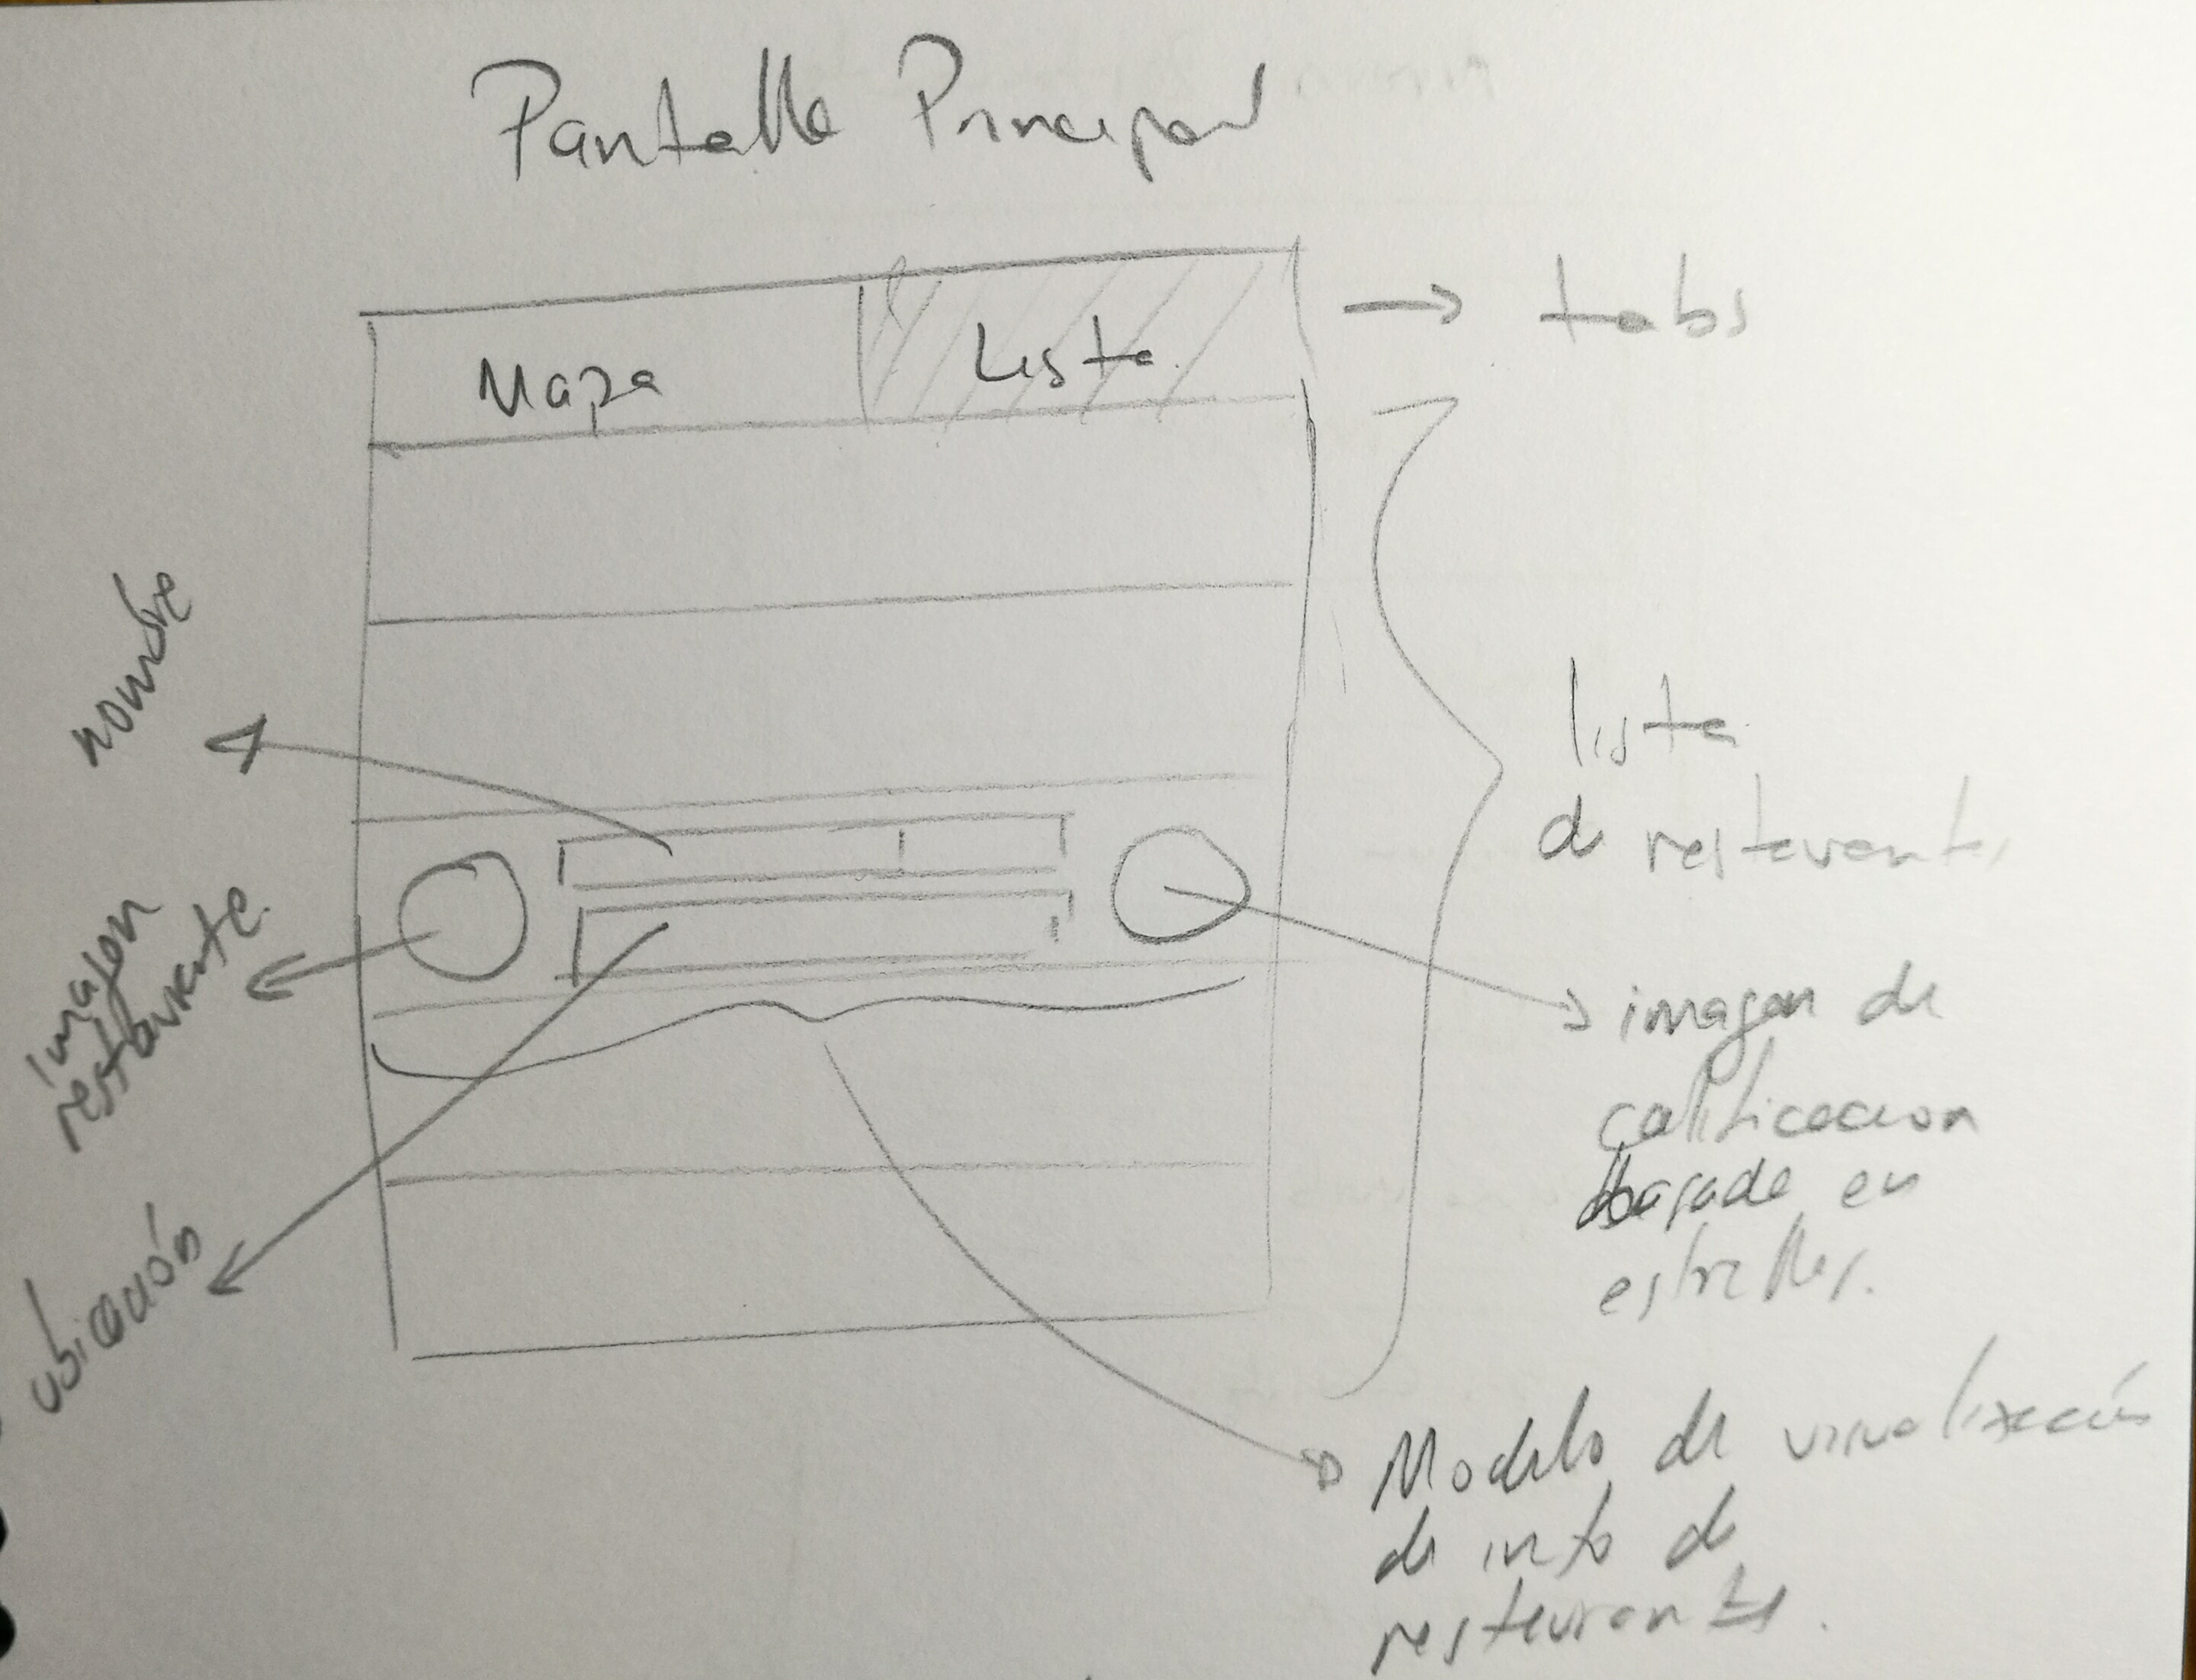
\includegraphics[scale=0.07]{pantalla_principal.jpg}
		\caption{Pantalla principal. Fuente: propia}
		\label{img:pantalla_principal}
	\end{center}
\end{figure}

\subsection{Pantalla para detalles del restaurante}
Esta pantalla muestran la información correspondiente al restaurante seleccionado. Primero se muestra el nombre del restaurante seguido por las fotos que los usuarios han ingresado. Posteriormente mediante el uso de estrella se indica la puntuación promedio de este, además se indica mediante algún ícono el precio general de la comida. Seguido se muestra la información como teléfono, tipo de comida que venden y horarios. Luego se muestra en un mapa la ubicación del restaurante. En esta pantalla se permite al usuario ingresar un comentario, por lo que se incluye un conjunto de estrellas para que el usuario pueda dar su calificación, de igual manera se maneja la calificación del precio, por último se tiene un cuadro de texto para indicar el comentario. Como último elemento de la pantalla, se tiene una lista de los comentarios que los usuarios han realizado de dicho restaurante.

\begin{figure}[h!]
	\begin{center}
		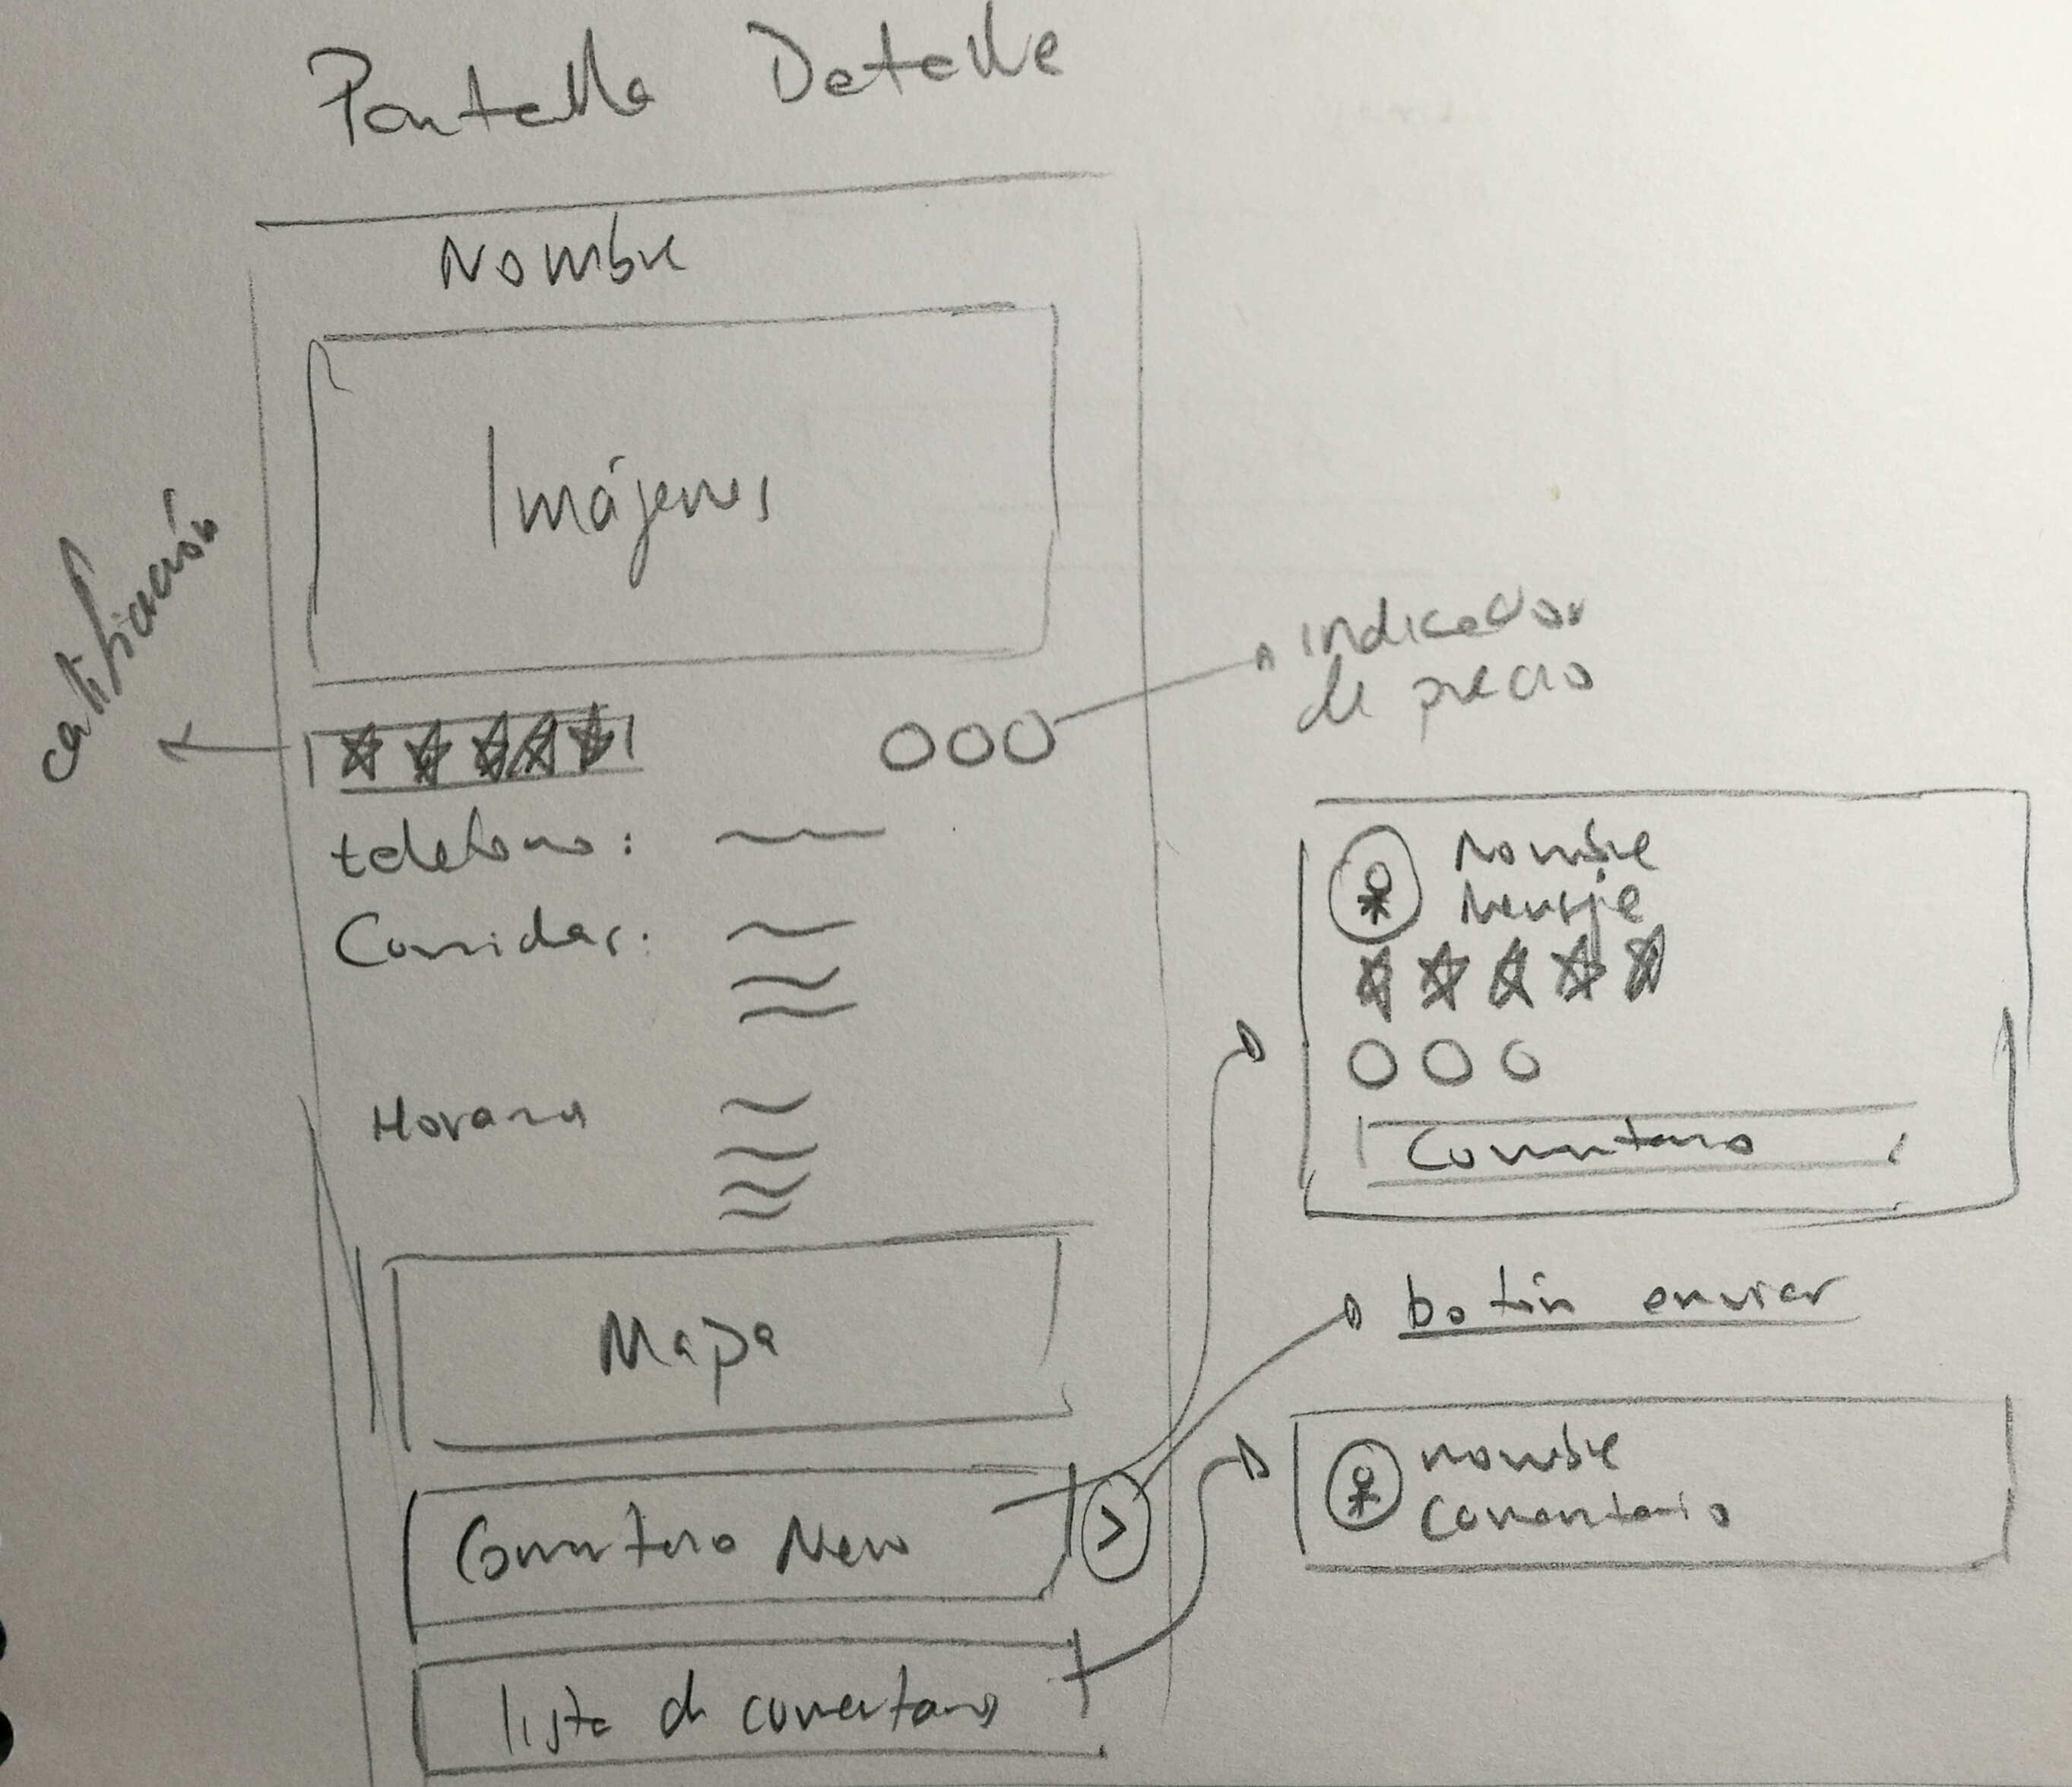
\includegraphics[scale=0.09]{pantalla_detalle.jpg}
		\caption{Pantalla para detalles del restaurante. Fuente: propia}
		\label{img:pantalla_detalles}
	\end{center}
\end{figure}

\section{Diseño de alto nivel de la aplicación}

\begin{figure}[h!]
	\begin{center}
		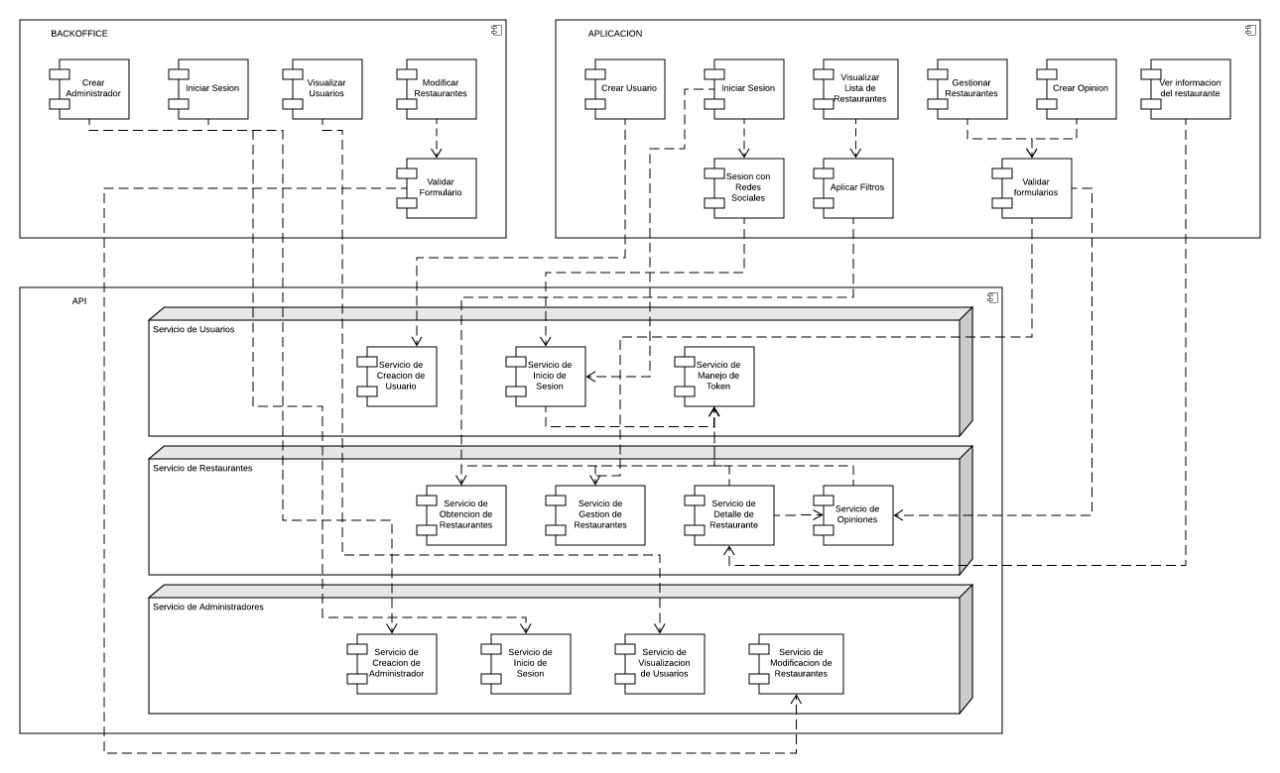
\includegraphics[scale=0.35]{diagrama_alto_nivel.jpeg}
		\caption{Diagrama para el desarrollo de la aplicación. Fuente: propia}
		\label{img:diagrama}
	\end{center}
\end{figure}

\section{Web service}

La implementación del API para la aplicación fue desarrollada utilizando Node.js mediante la creación de las rutas necesarias para suplir las funcionalidad de la aplicación, entre las que están la creación, modificación y consulta de restaurantes, el manejo de usuarios con respecto a la creación y login, así como el manejo de comentarios, entre otras cosas.

Este API fue desplegado utilizando la plataforma Heroku por su sencillez de implementación, así como por ser gratuita. La ruta utilizada por el API es \textbf{https://foodcourtec.herokuapp.com/}

Las siguiente secciones muestran los módulos en los que se dividieron las funcionalidades y rutas utilizadas por el API.

\subsection{Usuarios} 
\subsubsection{Registro de usuario: /createUser}
\noindent
\textbf{Envío: }\\
\noindent
\{ \\
``email'': ``Email del usuario'' \\
``name'': ``Nombre del usuario''\\
``password'': ``Contraseña del usuario''\\
\}

\noindent
\textbf{Respuesta: }\\
\noindent
\{ \\
``status'': ``Mensaje según lo sucedido'' \\
\}

\subsubsection{Registro de usuario: /loginUser}
\noindent
\textbf{Envío: }\\
\noindent
\{ \\
``email'': ``Email del usuario'' \\
``name'': ``Nombre del usuario''\\
``SocialLogin'': Boolean si el usuario ingresa con Facebook\\
\}

En este caso, si se inicia sesión con Facebook, la key ``password'' no es necesaria, igual en caso contrario.


\noindent
\textbf{Respuesta: }\\
\noindent
\{ \\
``token'': ``Token para las próximas solicitudes'' \\
``name'': ``Nombre del usuario'' \\
``photo'': ``Información binaria de la foto'' \\
``contentType'': ``Formato de la foto'' \\
\}

Si el inicio de sesión es por Facebook se recibirán únicamente el Token como respuesta.

\subsubsection{Registro de usuario: /requestCode}
\noindent
\textbf{Envío: }\\
\noindent
\{ \\
``email'': ``Email del usuario'' \\
\}

\noindent
\textbf{Respuesta: }\\
\noindent
\{ \\
``status'': ``Mensaje según lo sucedido'' \\
\}

Recordar que se envía un correo al email brindado con el código para cambiar la contraseña.

\subsubsection{Registro de usuario: /resetPassword}
\noindent
\textbf{Envío: }\\
\noindent
\{ \\
``email'': ``Email del usuario'' \\
``password'': ``Contraseña nueva'' \\
``code'': ``Código enviado al correo'' \\
\}

\noindent
\textbf{Respuesta: }\\
\noindent
\{ \\
``status'': ``Mensaje según lo sucedido'' \\
\}

\subsubsection{Registro de usuario: /updateName}
\noindent
\textbf{Envío: }\\
\noindent
\{ \\
``email'': ``Email del usuario'' \\
``token'': ``Token para solicitudes'' \\
``name'': ``Nuevo nombre'' \\
\}

\noindent
\textbf{Respuesta: }\\
\noindent
\{ \\
``token'': ``Token de repuesta'' \\
``status'': ``Mensaje según lo sucedido'' \\
\}

\subsubsection{Registro de usuario: /updatePhoto}
\noindent
\textbf{Envío: }\\
\noindent
\{ \\
``token'': ``Token para solicitudes'' \\
``email'': ``Email del usuario'' \\
``contentType'': ``Formato de la imagen'' \\
``avatar'': ``Imagen a colocar'' \\
\}

\noindent
\textbf{Respuesta: }\\
\noindent
\{ \\
``token'': ``Token de repuesta'' \\
``status'': ``Mensaje según lo sucedido'' \\
\}

\subsection{Comidas}
\subsubsection{Registro de usuario: /getFoods}
\noindent
\textbf{Envío: }\\
\noindent
\{ \\
``token'': ``Token para solicitudes'' \\
``email'': ``Email del usuario'' \\
\}

\noindent
\textbf{Respuesta: }\\
\noindent
\{ \\
``token'': ``Token de repuesta'' \\
``foods'': Comidas \\
\}

\subsection{Restaurantes}
Para los horarios, el array debe tener un tamaño exacto de 7 y cada dia debe tener el formato indicado.

\subsubsection{Registro de usuario: /createRestaurant}
\noindent
\textbf{Envío: }\\
\noindent
\{ \\
``token'': ``Token para solicitudes'' \\
``email'': ``Email del usuario'' \\
``name'': ``Nombre del restaurante'' \\
``address'': \{ ``lat'': Punto, ``long'': Punto, ``direction'': ``Descripción de la ubicación'' \} \\
Opcional ``number'': teléfono del restaurante \\
Opcional ``webPage'': ``Página web'' \\
Opcional ``foods'': Array de comidas \\
Opcional ``schedules'': [\{ ``day'': String, ``open'': Date, ``close'': Date \}] \\
\} \\ \\
\noindent
\textbf{Respuesta: }\\
\noindent
\{ \\
``token'': ``Token de repuesta'' \\
``status'': ``Mensaje según lo sucedido'' \\
``id'': ``id del restaurante''\\
\}

\subsubsection{Registro de usuario: /updateRestaurant}
\noindent
\textbf{Envío: }\\
\noindent
\{ \\
``token'': ``Token para solicitudes'' \\
``email'': ``Email del usuario'' \\
``id'': ``id del restaurante''\\
Opcional ``name'': teléfono del restaurante \\
Opcional ``number'': teléfono del restaurante \\
Opcional ``webPage'': ``Página web'' \\
Opcional ``foods'': Array de comidas \\
Opcional ``schedules'': [\{ ``day'': String, ``open'': Date, ``close'': Date \}] \\
\} \\ \\
\noindent
\textbf{Respuesta: }\\
\noindent
\{ \\
``token'': ``Token de repuesta'' \\
``status'': ``Mensaje según lo sucedido'' \\
\}

\subsubsection{Registro de usuario: /createOpinion}
\noindent
\textbf{Envío: }\\
\noindent
\{ \\
``token'': ``Token para solicitudes'' \\
``email'': ``Email del usuario'' \\
``id'': ``id del restaurante''\\
``opinion'': \{ ``qualification'': número, ``price'': número, ``date'': fecha, opcional ``comment'': ``Comentario del usuario'' \} \\
\} \\ 
\noindent
\textbf{Respuesta: }\\
\noindent
\{ \\
``token'': ``Token de repuesta'' \\
``status'': ``Mensaje según lo sucedido'' \\
\}

\subsubsection{Registro de usuario: /getOpinions}
\noindent
\textbf{Envío: }\\
\noindent
\{ \\
``token'': ``Token para solicitudes'' \\
``email'': ``Email del usuario'' \\
``id'': ``id del restaurante''\\
\} \\ 
\noindent
\textbf{Respuesta: }\\
\noindent
\{ \\
``token'': ``Token de repuesta'' \\
``opinions'': Array de opiniones\\
``status'': ``Mensaje según lo sucedido'' \\
\}

\subsubsection{Registro de usuario: /addPhoto}
Recordar que varios archivos se pueden asociar a una llave("photos") simultáneamente, si no el servidor no obtendrá las imágenes.

\noindent
\textbf{Envío: }\\
\noindent
\{ \\
``token'': ``Token para solicitudes'' \\
``email'': ``Email del usuario'' \\
``id'': ``id del restaurante''\\
``photos'': imágenes del restaurante (máximo 5)\\
\} \\ 
\noindent
\textbf{Respuesta: }\\
\noindent
\{ \\
``token'': ``Token de repuesta'' \\
``status'': ``Mensaje según lo sucedido'' \\
\}

\subsubsection{Registro de usuario: /getPhotos}
\noindent
\textbf{Envío: }\\
\noindent
\{ \\
``token'': ``Token para solicitudes'' \\
``email'': ``Email del usuario'' \\
``id'': ``id del restaurante''\\
\} \\ 
\noindent
\textbf{Respuesta: }\\
\noindent
\{ \\
``token'': ``Token de repuesta'' \\
``photos'': Array con la información binaria de las fotos\\
``status'': ``Mensaje según lo sucedido'' \\
\}

\subsubsection{Registro de usuario: /getRestaurants}
\noindent
\textbf{Envío: }\\
\noindent
\{ \\
``token'': ``Token para solicitudes'' \\
``email'': ``Email del usuario'' \\
``filter'': json con los filtros (indicados más adelante)\\
\} \\ 

\textbf{Formato Json con los filtros}

\noindent
\textbf{Envío: }\\
\noindent
\{ \\
Opcional ``price'': \{ ``min'': número, ``max'': número\} \\
Opcional ``qualification'': \{ ``min'': número, ``max'': número\} \\
Opcional ``location'': \{ ``lat'': número, ``long'': número, ``distance'': número\} \\
Opcional ``foods'': Array de comidas permitidas \\
\} \\ 

\noindent
\textbf{Respuesta: }\\
\noindent
\{ \\
``token'': ``Token de repuesta'' \\
``restaurants'': Array con los restaurantes\\
``status'': ``Mensaje según lo sucedido'' \\
\}


\section{Interacción con sistemas externos}
Para que se tenga un correcto funcionamiento de la aplicación desarrollada se requiere de tres sistemas independientes. El primero de ellos es el \textbf{API de Google Maps}, esta es utilizada para desplegar los marcadores de los restaurantes para que el usuario pueda de una manera visual buscar y seleccionar los restaurantes de interés. Por otro lado, se tiene el \textbf{API desarrollada para esta aplicación}, esta se encarga de responder todas las solicitudes de creación, modificación y consulta de los datos presentes en la base de datos, lo que nos lleva al tercer elemento requerido en esta aplicación. Este es la base de datos desarrollada en \textbf{MongoDB}.


\end{document}
